\documentclass[11pt,a4paper]{article}
\usepackage[margin=1in]{geometry}
\usepackage{graphicx}
\title{Q1\_DISTRIBUTION\_2026-03-08\\Scientific Milestone Report}
\author{Science-Chief}
\date{2026-03-08}
\begin{document}
\maketitle

\section*{1. Scope}
This report documents the Q1 activity-distribution milestone: empirical distribution $P(k)$ of feedback count per agent.

\section*{2. Data Provenance and Purpose}
Data originate from ERC8004 Ethereum registries:
Identity Registry \texttt{0x8004A169FB4a3325136EB29fA0ceB6D2e539a432}, Reputation Registry \texttt{0x8004BAa17C55a88189AE136b182e5fdA19dE9b63}.
We extract these events to test whether agent feedback activity is heavy-tailed and to quantify concentration in participation.

\section*{3. Extraction and Variable Definition}
From \texttt{reputation\_newfeedback.csv}, we compute for each agent $k=$ number of received feedback events. The object of interest is $P(k)$, i.e., the fraction (or count) of agents with activity level $k$.

\section*{4. Results}
\begin{figure}[htbp]
\centering
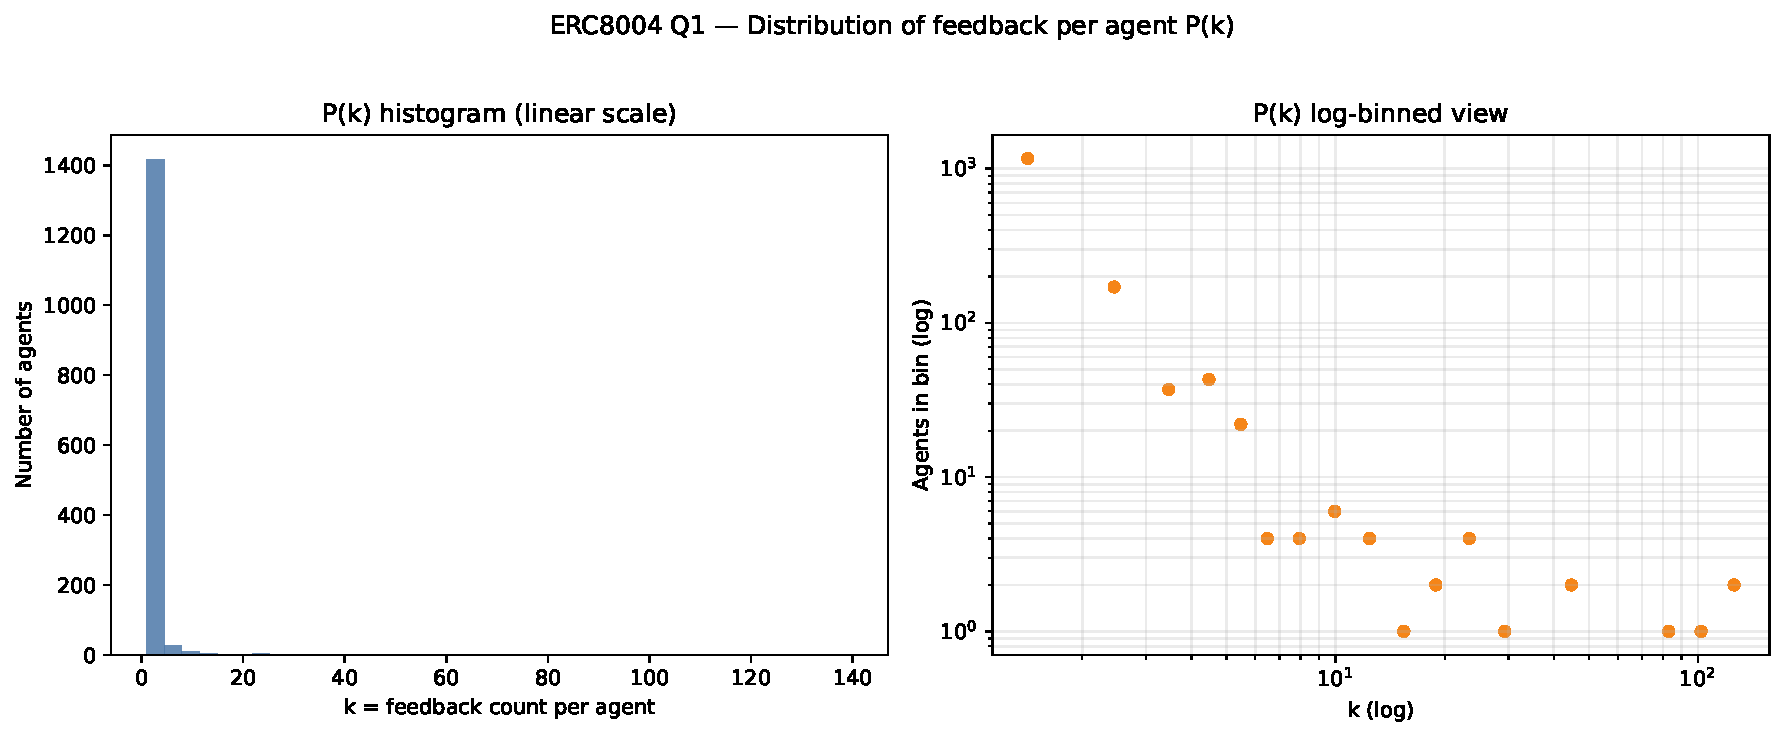
\includegraphics[width=0.88\textwidth]{figures/q1_pk_distribution_fast.pdf}
\caption{Preliminary empirical activity distribution $P(k)$.}
\end{figure}
The curve is right-skewed, with many low-activity agents and a long upper tail.

\section*{5. Limitations and Interpretation}
Current evidence is exploratory only. A formal power-law claim requires explicit fit parameters ($\alpha$, $x_{min}$), goodness-of-fit tests, and model comparison against alternatives (lognormal/exponential).

\section*{6. Decision and Next Actions}
\textbf{Decision: GO internal continuation, HOLD external claim.}
Next: complete inferential model-selection package and publish decision table.

\section*{Appendix: Source Paths}
\textbf{Figures}\\
\begin{itemize}
\item \texttt{workspaces/science-chief/outbox/Reports/Q1\_DISTRIBUTION\_2026-03-08/figures/q1\_pk\_distribution\_fast.pdf}
\end{itemize}

\end{document}
